\chapter{Manual técnico}
\section{Entorno de desenvolvemento}
Se ben non é necesario o uso de ningún entorno de desenvolvemento integrado (IDE) para a modificación do código do plugin, si é recomendable para aumentar a produtividade gracias as funcionalidades como o resaltado de sintaxe, o autocompletado ou a validación automática do código.

A continuación descríbense os pasos a seguir para a instalación dun entorno de desenvolvemento integrado igual ó empregado para a realización do plugin, que se levou a cabo sobre o sistema operativo Ubuntu.

O IDE recomendado na propia documentación de QGIS para o desenvolvemento de plugins en Python é Eclipse\footnote{\url{https://eclipse.org/}} co plugin PyDev\footnote{\url{http://pydev.org/}}, que pode instalarse dende o propio Eclipse. Amais do plugin PyDev tamén debemos instalar o plugin EGit para descargar o código dende GitHub. Tamén debemos ter instalado no equipo o QGIS, que se pode instalar desde os propios repositorios de Ubuntu, o igual que o Eclipse.

Para crear un proxecto desde o repositorio de GitHub existen varias opcións, a máis sinxela sería a seguinte:
\begin{itemize}
\item Seleccionar a opción de Import no menú File, e posteriormente Projects from Git.
\begin{figure}[H]
\centering
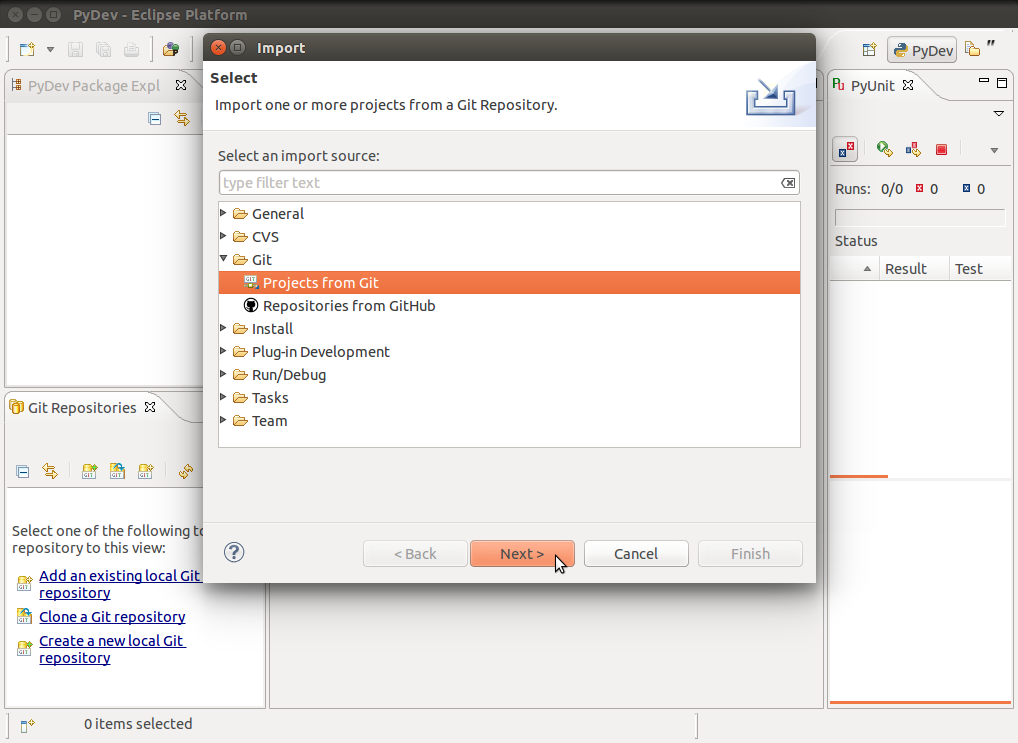
\includegraphics[width=0.8\textwidth]{images/manualtecnico/import_project01.png}
\caption{Importación do repositorio en Eclipse, paso 1}
\label{fig:import_project01}
\end{figure}
\item Seleccionar a opción GitHub e buscar o repositorio SOS Client.
\begin{figure}[H]
\centering
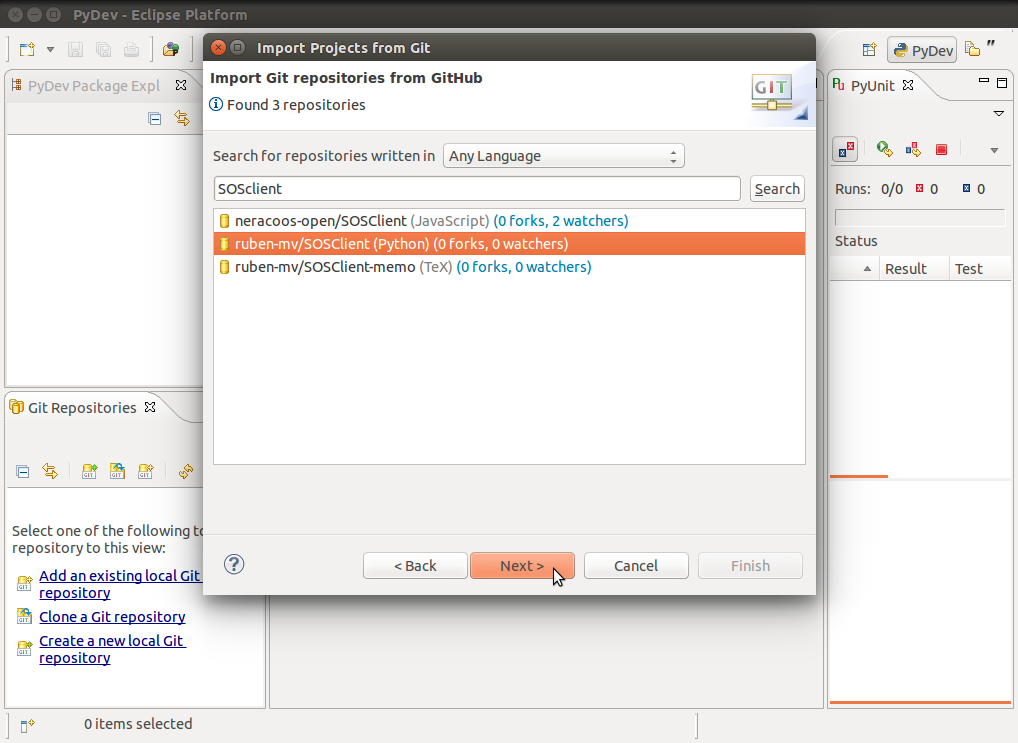
\includegraphics[width=0.8\textwidth]{images/manualtecnico/import_project02.png}
\caption{Importación do repositorio en Eclipse, paso 2}
\label{fig:import_project02}
\end{figure}
\item Engadir a rama master e importar coa opción Import as general project.
\begin{figure}[H]
\centering
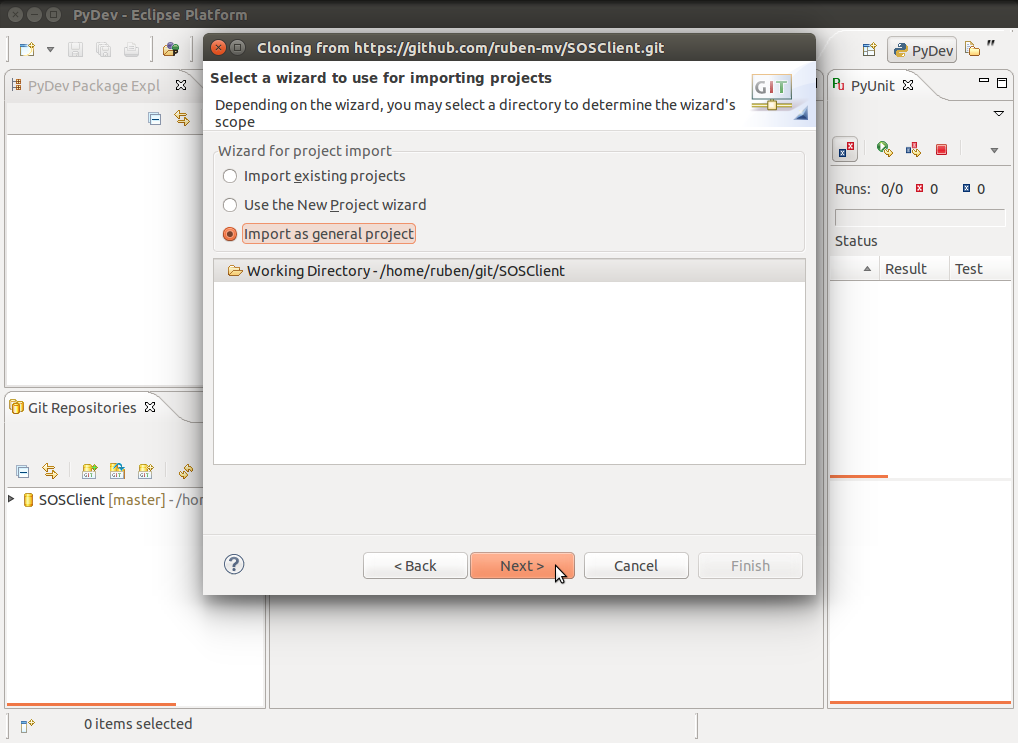
\includegraphics[width=0.8\textwidth]{images/manualtecnico/import_project03.png}
\caption{Importación do repositorio en Eclipse, paso 3}
\label{fig:import_project03}
\end{figure}
\item Unha vez feito importado o proxecto pódese converter nun proxecto de PyDev.
\begin{figure}[H]
\centering
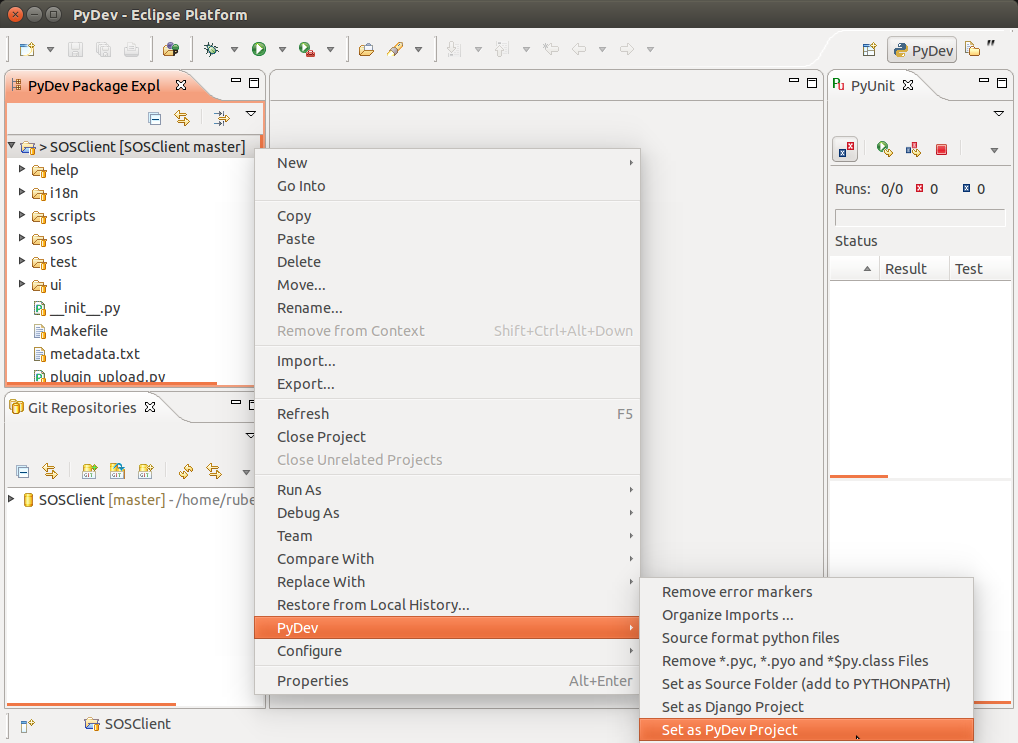
\includegraphics[width=0.8\textwidth]{images/manualtecnico/import_project04.png}
\caption{Importación do repositorio en Eclipse, paso 4}
\label{fig:import_project04}
\end{figure}
\end{itemize}

A continuación débese configurar o PyDev para que recoñeza a API de QGIS e de PyQt4 de forma que teñamos dispoñibles as funcións de autocompletado. Para esto, dende a ventá de Window $\to$ Preferences accedese á configuración do interprete de Python, onde haberá que engadir na lapela de librerías a carpeta $\sim$/.qgis/python/plugins/, e na lapela Forced builtin engadir qgis e PyQt4.
\begin{figure}[H]
\centering
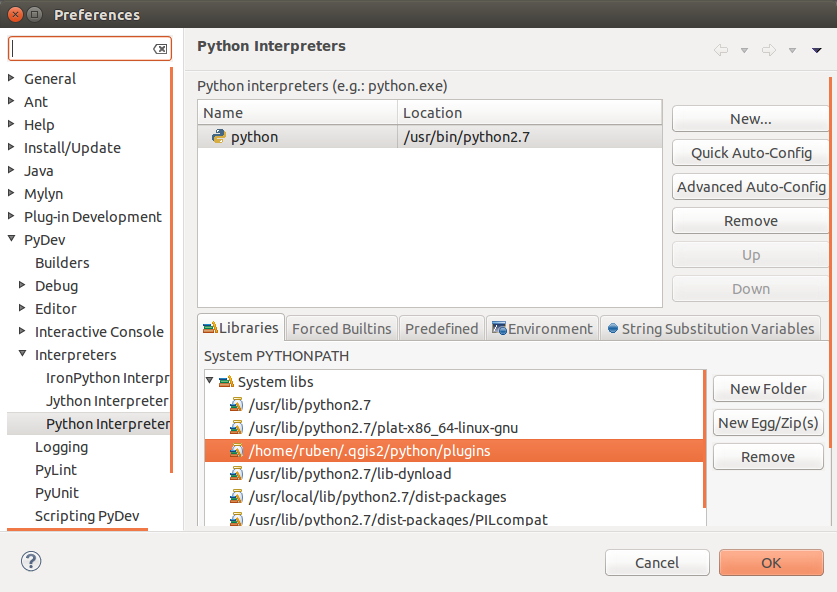
\includegraphics[width=0.8\textwidth]{images/manualtecnico/python_settings.png}
\caption{Configuración de Python en Eclipse}
\label{fig:python_settings}
\end{figure}

Tamén se deben engadir as carpetas do proxecto ó PYTHONPATH, desde as propiedades do proxecto:
\begin{figure}[H]
\centering
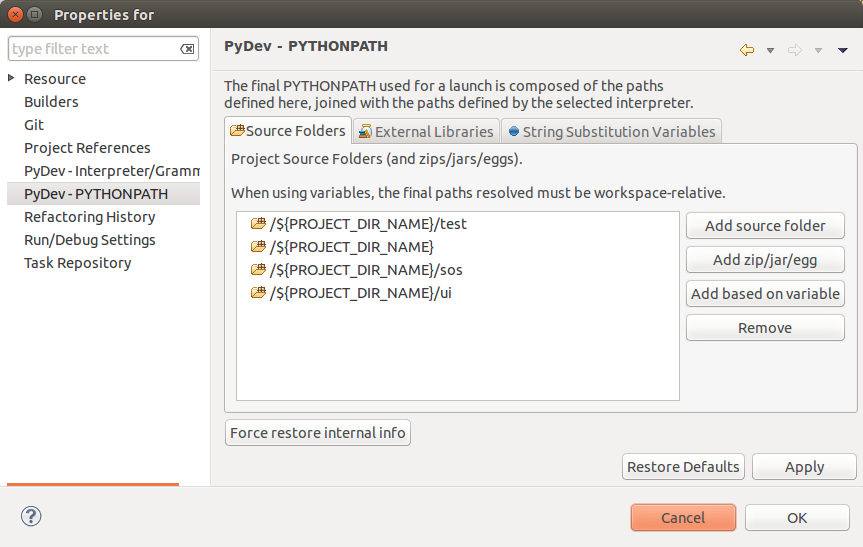
\includegraphics[width=0.8\textwidth]{images/manualtecnico/python_path.png}
\caption{Configuración do PYTHONPATH}
\label{fig:python_path}
\end{figure}


O proxecto foi creado inicialmente co plugin 'Plugin Builder'\footnote{\url{http://g-sherman.github.io/Qgis-Plugin-Builder/}} de QGIS polo que contén un Makefile que nos permite usar make coas seguintes opcións, entre outras:
\begin{description}
\item[deploy:] Desprega o plugin na carpeta correspondente.
\item[derase:] Elimina a carpeta de despregue do plugin.
\item[transup:] Actualiza os ficheiros de traducións.
\item[zip:] Desprega o plugin e crea un zip axeitado para subir ó repositorio de QGIS.
\item[test:] Executa os tests.
\end{description}

Tamén é de moita utilidade instalar no QGIS o plugin 'Plugin Reloader'\footnote{\url{http://plugins.qgis.org/plugins/plugin_reloader/}}, que se pode instalar dende o propio menú do QGIS. Este plugin permite volver a cargar un plugin dende disco sen necesidade de cerrar e volver a abrir o QGIS.

Outras ferramentas que se poden necesitar para o desenvolvemento do plugin son o QtDesigner, para modificar os ficheiros ui nos que se define a interface gráfica, e o QtLingüist, para as traducións a distintos idiomas.

\section{Ampliación do módulo de procesamento XML}
TODO: Documentar como ampliar o parser de XML para engadir soporte de máis implementacións do SOS.